\section{Configuration and Computation History}

Recall that the \textit{\textbf{configuration}} of a Turing machine can be expressed as a triple $(q,p,t)$ where $q$ is the current state, $p$ is the head position, and $t$ is the tape content. Equivalently, this can be written as an encoding $t_1qt_2$ where $t = t_1t_2$ and the head position is on the first symbol of $t_2$.

\begin{example}[Configuration of a Turing Machine]
    For example, the configuration 
    $$(q_3,6,aaaaaabbbbb)$$
    means the Turing machine is in state $q_3$, with the head pointing at the 6th symbol, and the current tape content being $aaaaaabbbbb$. This can be expressed in a more compact form as
    $$
    aaaaa q_3 abbbbb
    $$
\end{example}

A computation history of a Turing machine is a sequence of configurations of the Turing machine until it reaches an accepting state.

\begin{definition}[Computation History]
    An \textit{\textbf{accepting computation history}}, or \textit{\textbf{computation history}}, for a Turing machine $M$ on input $w$ is a sequence of configurations $C_1,C_2,\ldots,C_{accept}$ that $M$ enters until it accepts. Each configuration in this sequence is yielded from the configuration immediately before it.
    
    We encode a computation history as a sequence of configurations separated by the pound sign \#.
    $$
    C_1 \# C_2 \# \ldots \# C_{accept}
    $$
\end{definition}

\begin{example}
    A computation history for $M$ on $w = w_1w_2\ldots w_n$ given $\delta(q_0,w_1) = \delta(q_7,a,R)$ and $\delta(q_7,w_2) = (q_8,c,R)$ is as follows
    $$
    \underbrace{q_0w_1w_1 \ldots w_n}_{C_1} \# \underbrace{aq_7w_2 \ldots w_n}_{C_2} \# \underbrace{acq_8w_3 \ldots w_n}_{C_3} \# \cdots \# \underbrace{\ldots q_{accept} \ldots}_{C_{accept}}
    $$
\end{example}

\section{Decidability of Problems Concerning Linearly Bounded Automata}

To understand how to prove undecidability using the computation history method, we first examine a type of machine known as linearly bounded automata (LBA).

\begin{definition}[Linearly Bounded Automaton]
    A \textit{\textbf{linearly bounded automaton (LBA)}} is a single-tape Turing machine that cannot move its head off the input portion of the tape. In other words, the size of the tape is restricted to the size of the input.
\end{definition}

\subsection{A\textsubscript{LBA} is Decidable}

Let
$$
\A_{\LBA} = \{ \encoding{B,w} \mid \text{LBA $B$ accepts $w$} \}
$$
Although it may come as surprising at a first glance, $\A_{\LBA}$ is, in fact, decidable. This is because of the fac that, for an LBA of input size $n$, the number of configurations of the LBA is finite, namely equal to $|Q| \times n \times |\Gamma|^n$.

\textit{Claim}. For inputs of length $n$, an LBA can only have $|Q| \times n \times |\Gamma|^n$ configurations.

\begin{theorem}
    $\A_{\LBA}$ is decidable.
\end{theorem}

\begin{proof}
    If $B$ on $w$ runs for too long (more than $|Q| \times n \times |\Gamma|^n$), then by the pigeonhole principle, $B$ must be looping and will never halts or accept. More formally, let us construct a decider for $\A_{\LBA}$.
    $$
    \begin{aligned}
        D_{\A_{\LBA}} = 
            `` &\text{on input $\encoding{B,w}$} \\
            &\text{1. Let $n = |w|$} \\
            &\text{2. Run $B$ on $w$ for $|Q| \times n \times |\Gamma|^n$ steps} \\
            &\text{3. If $B$ has accepted, accept} \\
            &\text{4. If $B$ has rejected or it is still running, reject}
            ''
    \end{aligned}
    $$
\end{proof}

\subsection{E\textsubscript{LBA} is Undecidable}
Now, let us consider the language
$$
\E_{\LBA} = \{ \encoding{B} \mid \text{$B$ is an LBA and $\lang(B) = \emptyset$} \}
$$
The next natural question is whether or not $\E_{\LBA}$ is also decidable. We will show using reduction that $\ATM$ can be reduced to $\E_{\LBA}$ and thus $\E_{\LBA}$ is undecidable.

\begin{theorem}
    $\E_{\LBA}$ is undecidable.
\end{theorem}

\begin{proof}
    Assume that $\E_{\LBA}$ is decidable. Then, there exists a Turing machine $R$ that decides $\E_{\LBA}$. We construct a Turing machine $S$ deciding $\ATM$.
    $$
    \begin{aligned}
        S = 
            `` &\text{on input $\encoding{M,w}$} \\
            &
            \begin{aligned}
                \text{1. } &\text{Construct LBA $B_{\encoding{M,w}}$ that tests whether its input $x$ is an accepting computation history} \\
                &\text{for $M$ on $w$, and accepts only if $x$ is an accepting computation history}
            \end{aligned} \\
            &\text{2. Use $R$ to determine whether $\lang(B_{\encoding{M,w}}) = \emptyset$} \\
            &\text{3. Accept if no. Reject if yes.}
            ''
    \end{aligned}
    $$
    More specifically, we define $B_{\encoding{M,w}}$ as follows.
    $$
    \begin{aligned}
        B_{\encoding{M,w}} = 
        `` &\text{on input $x$} \\
        &\text{1. Check if $x$ begins $C_1 \#$ where $C_1$ is the start configuration of $M$ on $w$} \\
        &\text{2. Check if each $C_{i+1}$ yields from $C_i$ } \\
        &\text{3. Check if the final configuration is accepting} \\
        &\text{4. Accept if all checks pass. Otherwise, reject.}
    \end{aligned}
    $$
    Clearly, $S$ accepts if and only if $M$ on $w$ accepts, and it halts on all inputs. Hence, $S$ decides $\ATM$, but since $\ATM$ is undecidable, this is a contradiction.
\end{proof}

\section{Post Correspondence Problem}

A domino has the form $\displaystyle \left[ \frac{t}{b} \right] $ where $t, b \in \Sigma^*$.

Given a collection of dominos $\displaystyle P = \left\{ \left[ \frac{t_1}{b_1} \right], \ldots, \left[ \frac{t_k}{b_k} \right] \right\}$, we say there is a \textit{\textbf{match}} if we can make a list using the dominos from $P$ (possibly with repetitions) such that the whole string on the top row is equal to the whole string on the bottom row. The \textit{\textbf{Post Correspondence Problem (PCP)}} is to determine whether a collection of dominos $P$ has a match.

Figure \ref{fig:pcp-example} shows a set of dominos and a match.

\begin{figure}[htbp]
    \centering
    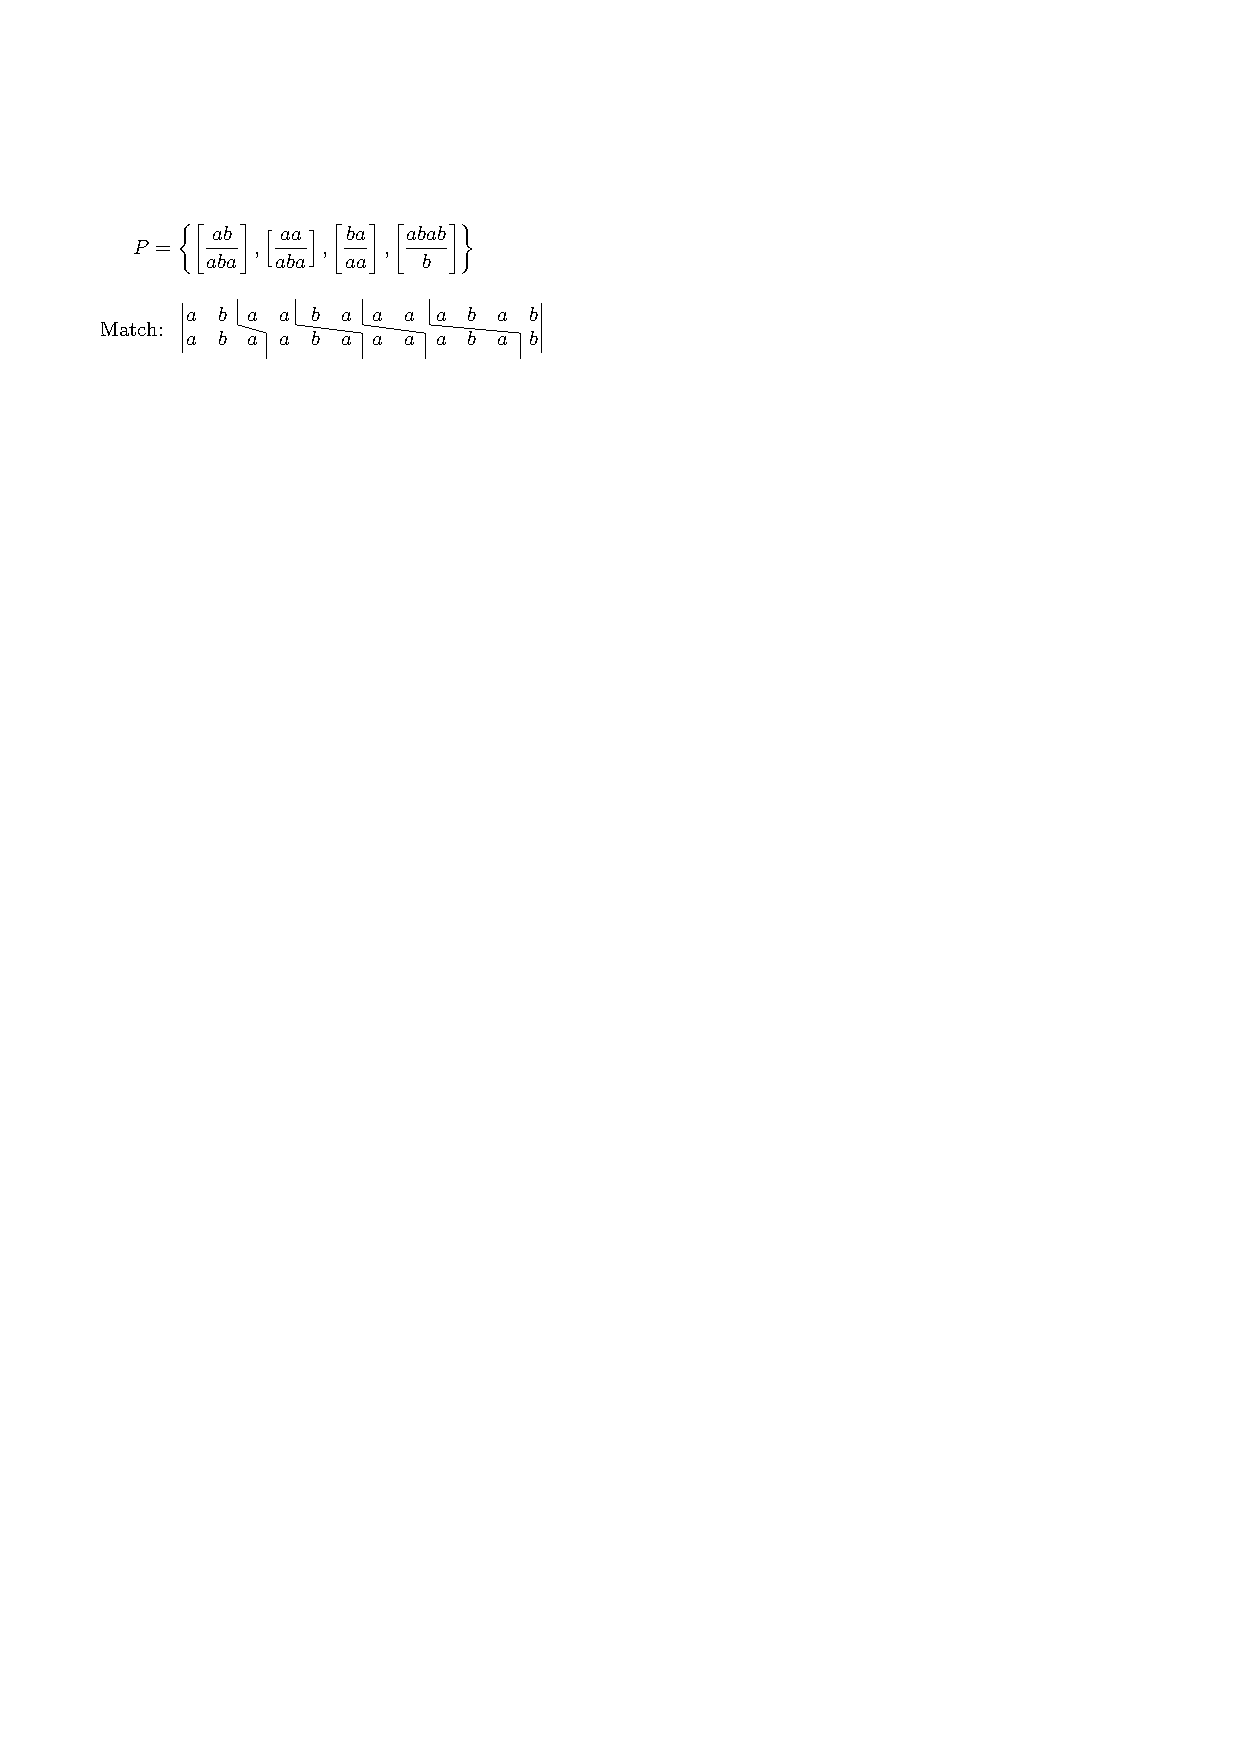
\includegraphics[width=0.6\linewidth]{pcp-example.pdf}
    \caption{A set of dominos $P$ and the corresponding match.}
    \label{fig:pcp-example}
\end{figure}

\begin{theorem}
    $\PCP$ is undecidable.
\end{theorem}

The main idea of the proof: reduction $\ATM \leq_m \PCP$ using computation histories. We will in fact show two reductions:
$$
\ATM \leq_m \MPCP \leq_m \PCP
$$

To make the proof simpler, we first restrict ourselves to the Modified Post Correspondence Problem (MPCP). MPCP adds the additional requirement that the match starts with the first domino $\left[ \frac{t_1}{b_1} \right]$.